\chapter{\sc Two-Phase Navier--Stokes Flow Numerical Results}
\label{ch:ns_results}

\section{Exact solutions}\label{sec:ns_exact_solutions}
In order to test our method, we recall the following expanding spherical
solutions. Let $\Gamma(t) = \{ \vec z \in \R^d : |\vec z| = r(t)\}$ be a sphere
of radius $r(t)$ and curvature $\kappa(t) = -\,\frac{d-1}{r(t)}$. Moreover let
$\alpha,\alpha_1,\alpha_2,\gamma\in \R_{\geq 0}$ be given. Here, we also allow
non divergence-free problem. Therefore, in the continuous model
(\ref{eq:ns_full_momentum}--i), the incompressibility condition
(\ref{eq:ns_full_mass}) is replaced by
\begin{equation}\label{eq:ns_compressible}
\nabla\,.\,\vec u = f_{\rm{div}}\,.
\end{equation}

Firstly, the expanding sphere where
\begin{equation} \label{eq:r_benchmark1}
r(t) = \mathrm{e}^{\alpha\,t}\,r(0)\,,
\end{equation}
together with
\begin{equation} \label{eq:up_benchmark1}
\vec u(\vec z, t) = \alpha\,\vec z \,, \quad
p(\vec z, t) = -\,\bigg(\gamma - 2\,\alpha\,\frac{\mu_+ - \mu_-}
{d-1}r(t)\bigg)\,\kappa(t)\,\left[ \charfcn{\Omega_-(t)} -
\frac{\vol(\Omega_-(t))}{\vol(\Omega)}\right],
\end{equation}
is an exact solution to the problem (\ref{eq:ns_full_momentum}--i), with
(\ref{eq:ns_full_mass}) replaced by (\ref{eq:ns_compressible}), on
e.g.\ $\Omega = (-1,1)^d$  with $\vec f(\vec z, t) = \rho\,\alpha^2\,\vec z$,
$f_{\rm{div}} = \alpha\,d$ and $\vec g = \alpha\,\vec z$ on
$\partial_1\Omega=\partial\Omega$.

Alternatively, the expanding sphere where
\begin{equation} \label{eq:r_benchmark2}
r(t) = \mathrm{e}^{\alpha_1\,t}\,r(0)\,,
\end{equation}
together with
\begin{align} \label{eq:up_benchmark2}
& \vec u(\vec z, t) = \bigg(\alpha_1+\alpha_2\charfcn{\Omega_+(t)}(|\vec
z|^2-r(t)^2)\bigg)\,\vec z\,, \\
& p(\vec z, t) = -\,\bigg(\gamma - 4\,\alpha_2\,\frac{\mu_+}{d-1}r(t)^3
\bigg)\,\kappa(t)\,\left[ \charfcn{\Omega_-(t)} -
\frac{\vol(\Omega_-(t))}{\vol(\Omega)}\right],
\end{align}
is an exact solution to the problem (\ref{eq:ns_full_momentum}--i), with
(\ref{eq:ns_full_mass}) replaced by (\ref{eq:ns_compressible}), on e.g.\ $\Omega
= (-1,1)^d$ with
\begin{align}
\vec f(\vec z, t) = &
\rho\,\bigg(\alpha_1^2\,+\charfcn{\Omega_+(t)}\bigg(-2\alpha_1\alpha_2r(t)^2 +
2\alpha_1\alpha_2\big(2|\vec z|^2-r(t)^2\big) \nonumber \\
& +\alpha_2^2\big(|\vec z|^2-r(t)^2\big)\big(3|\vec z|^2 -
r(t)^2\big)-4(d+1)\alpha_2\frac{\mu_+}{\rho}\bigg)\bigg)\vec z\,,
\end{align}
\begin{equation}
f_{\rm{div}} = \big( \alpha_1
+ \alpha_2\charfcn{\Omega_+(t)}\big(\frac{2+d}{d}|\vec z|^2-r(t)^2\big)\big)d
\end{equation}
and
\begin{equation}
\vec g = \bigg(\alpha_1+\alpha_2\charfcn{\Omega_+(t)}(|\vec
z|^2-r(t)^2)\bigg)\,\vec z
\end{equation}
on $\partial_1\Omega=\partial\Omega$.

Finally, a nontrivial divergence free and radially symmetric solution $\vec u$
can be constructed on a domain that does not contain the origin. To this end,
consider e.g.\ $\Omega = (-1,1)^d \setminus [-\frac13, \frac13]^d$. Then, the
expanding sphere where
\begin{equation} \label{eq:r_benchmark3}
r(t) = ([r(0)]^d + \alpha\,t\,d)^\frac1d \,,
\end{equation}
together with
\begin{equation} \label{eq:up_benchmark3}
\vec u(\vec z, t) = \alpha\,\frac{\vec z}{|\vec z\,|^d}\,, \quad
p(\vec z, t) = -\,\bigg(\gamma +2\,\alpha\,\frac{\mu_+ - \mu_-}
{r(t)^{d-1}}\bigg)\,\kappa(t)\,\left[ \charfcn{\Omega_-(t)} -
\frac{\vol(\Omega_-(t))}{\vol(\Omega)}\right],
\end{equation}
is an exact solution to the problem (\ref{eq:ns_full_momentum}--i) with
$\vec f(\vec z, t) = (1-d)\alpha^2\frac{\vec z}{|\vec z|^{2d}}$ and $\vec g(\vec
z) = \alpha\,|\vec z|^{-d}\,\vec z$ on $\partial_1\Omega=\partial\Omega$.

\section{Non divergence-free antisymmetric scheme}
Some exact solution presented in \S\ref{sec:ns_exact_solutions} are non
divergence-free which means that $\nabla\,.\,\vec u = f_{\rm{div}}$ in
$\Omega_\pm(t)$. Consequently, (\ref{eq:advect}) is no longer valid and we need
to use (\ref{eq:fulladvect}) to derive the antisymmetric weak formulation.
Therefore an additional term $\tfrac{1}{2}(\rho\,f_{\rm{div}}\,\vec
u,\vec\xi)$ appears in the momentum equation (\ref{eq:ns_weaka_antisym}).
Hence, the weak antisymmetric formulation (\ref{eq:ns_weaka_antisym}--d) is
replaced by
\begin{subequations}
\begin{align}
& \tfrac{1}{2}\bigg[ \ddt (\rho\,\vec u, \vec \xi) + (\rho\,\vec u_t, \vec \xi)
+ (\rho, [(\vec u\,.\,\nabla)\,\vec u]\,.\,\vec \xi
- [(\vec u\,.\,\nabla)\,\vec \xi]\,.\,\vec u) \bigg] \nonumber \\
& \qquad +2\left(\mu\,\mat D(\vec u), \mat D(\vec \xi)\right)
- \left(p, \nabla\,.\,\vec \xi\right)\nonumber \\
& \qquad - \gamma\,\left\langle \varkappa\,\vec\nu, \vec\xi
\right\rangle_{\Gamma(t)}
= \left(\vec f, \vec \xi\right)+(\rho\,f_{\rm{div}}\,\vec u,\vec\xi)
\quad \forall\ \vec\xi \in \uspace 0 \,,
\label{eq:ns_weaka_antisym_div}\\
& \left(\nabla\,.\,\vec u, \varphi\right) = f_{\rm{div}}
\quad \forall\ \varphi \in \pnormspace\,, \label{eq:ns_weakb_antisym_div} \\
&  \left\langle \V
- \vec u, \chi\,\vec\nu \right\rangle_{\Gamma(t)} = 0
\quad \forall\ \chi \in H^1(\Gamma(t))\,, \label{eq:ns_weakc_antisym_div} \\
& \left\langle \varkappa\,\vec\nu, \vec\eta \right\rangle_{\Gamma(t)}
+ \left\langle \nabs\,\vec \id, \nabs\,\vec \eta \right\rangle_{\Gamma(t)}
= 0  \quad \forall\ \vec\eta \in
[H^1(\Gamma(t))]^d\,.\label{eq:ns_weakd_antisym_div}
\end{align}
\end{subequations}

\section{Benchmark quantities}\label{sec:benchmark_quantities}
In our numerical simulations, unless otherwise stated, we use the following
settings. We choose the initial surface $\Gamma(0) = \{ \vec z \in \R^d : |\vec
z| = \frac12 \}$, the domain $\Omega = (-1,1)^d$ and we employ uniform time
steps $\tau_m=\tau$, $m=0,\ldots, M-1$. Moreover, we set the GMRES tolerance to
tol $=10^{-12}$ and the restart value to 50. We use the Stokes matrix
(\ref{eq:stokes_direct_precond}) or, depending on the pressure space,
(\ref{eq:stokes_direct_precond_extended}) as a preconditioner factorizing it
with UMFPACK. Moreover, we use the errors (\ref{eq:errorXx}),
(\ref{eq:errorLUu}), (\ref{eq:errorHUu}), (\ref{eq:errorPp}) and the estimated
error of convergence EOC (\ref{eq:eoc}). See \S\ref{sec:errors} for more
details.

For later use, we define some benchmark quantities for the continuous
solution $(\vec u, p, \Gamma)$ of (\ref{eq:ns_full_momentum}--i). Let
\begin{equation}
z_c(t) = \frac{1}{\vol(\Omega_-(t))}\int_{\Omega_-(t)} z_d \dL{d}
\end{equation}
denotes the $d$-component of the bubble's centre of mass, where $z_d$ is the
$d$-component of the position vector $\vec z$. Let $\strikes(t)$ denotes the
degree of sphericity of $\Gamma(t)$, which is defined as the ratio between the
surface volume of a volume-equivalent hypersphere and $\surfvol(\Gamma(t))$. Let
\begin{equation}
V_c(t) = \frac{1}{\vol(\Omega_-(t))}\int_{\Omega_-(t)} u_d(t) \dL{d}
\end{equation}
denotes the bubble's rise velocity, where $u_d(t)$ is the $d$-component of
$\vec u$. Therefore, the discrete counterpart of $d$-component of the bubble's
centre of mass is
\begin{equation}
z_c^m = \frac{1}{\vol(\Omega_-^m)}\,\int_{\Omega_-^m} z_d^{m} \dL{d}\,,
\end{equation}
while the degree of sphericity becomes
\begin{equation}
\strikes^m =\frac{\pi^{\frac{1}{d}}[2\,d\,\vol(\Omega_-^m)]^\frac{d-1}{d}}
{\surfvol(\Gamma^m)}\,
\end{equation}
and the bubble's rise velocity assumes the following form
\begin{equation}
V^m_c = \frac{1}{\vol(\Omega_-^m)}\,\int_{\Omega_-^m}U^m_d\dL{d}\,,
\end{equation}
where $U^m_d$ is the $d$-component of $\vec U^m$ evaluated on $\Omega^m$.

\section{Rising bubble experiment in 2d}\label{sec:2d_rising_bubble_results}
We use the same  setup described in \cite{HysingTKPBGT09}, see Figure~2 there,
which is ${\Omega = (0,1) \times (0,2)}$ with $\partial_1\Omega = [0,1] \times
\{0,2\}$ and $\partial_2\Omega = \{0,1\} \times (0,2)$. Moreover, let the
initial interface be ${\Gamma_0 = \{\vec z \in \R^2 : |\vec z - (\frac{1}{2},
\frac{1}{2})^T| = \frac{1}{4}\}}$. The physical parameters from the test case 1
in \cite[Table~I]{HysingTKPBGT09} are then given by
\begin{equation} \label{eq:Hysing1}
\rho_+ = 1000\,,\quad \rho_- = 100\,,\quad \mu_+ = 10\,,\quad \mu_- = 1\,,\quad
\gamma = 24.5\,,
\end{equation}
with $\vec f = -0.98\,\rho\,\vec e_2$ and $\vec g=\vec 0$. The time interval
chosen for the simulations is $[0,3]$, we adopt an uniform time step size
$\tau=10^{-3}$ and nearly uniform bulk meshes. Moreover, we set
$C_a=20$\textdegree, recall (\ref{eq:angle_criterion}).

We list our employed discretization parameters in
Table~\ref{tab:risingbubble2Delements}.
\begin{table*}
\center
\begin{tabular}{rrrrrr}
\hline
$J_\Gamma$ & $J_\Omega^0$ & $J_\Omega^M$ explicit & $J_\Omega^M$ implicit &
$J_\Omega^M$ antisymmetric & $J_\Omega^M$ ALE \\
\hline
 32 & & & & & \\
 64 & & & & & \\
128 & & & & & \\
\hline
\end{tabular}
\caption[Navier--Stokes 3d rising bubble meshes parameters]
{Discretization parameters for the 2d rising bubble experiment.}
\label{tab:risingbubble2Delements}
\end{table*}

\begin{table*}
\center
\hspace*{-3.25cm}
\begin{tabular}{rlll}
\hline
 & $J_\Gamma=32$ & $J_\Gamma=64$ & $J_\Gamma=128$ \\
\hline
& \multicolumn{3}{c}{explicit} \\
\cmidrule{2-4}
$\strikes_{\min}$                & 0.8986 & 0.9002 & 0.9007 \\
$t_{\strikes = \strikes_{\min}}$ & 2.1560 & 1.9450 & 1.9420 \\
$V_{c,\max}$                     & 0.2372 & 0.2402 & 0.2404 \\
$t_{V_c = V_{c,\max}}$           & 1.0190 & 0.9370 & 0.9250 \\
$z_c(t=3)$                       & 1.0857 & 1.0837 & 1.0816 \\
CPU                              &  13664 &  24539 & 211168 \\
\cmidrule{2-4}
& \multicolumn{3}{c}{implicit} \\
\cmidrule{2-4}
$\strikes_{\min}$                & 0.8986 & 0.8990 & 0.9011 \\
$t_{\strikes = \strikes_{\min}}$ & 2.1560 & 1.9190 & 1.8400 \\
$V_{c,\max}$                     & 0.2372 & 0.2402 & 0.2403 \\
$t_{V_c = V_{c,\max}}$           & 1.0190 & 0.9370 & 0.9240 \\
$z_c(t=3)$                       & 1.0857 & 1.0862 & 1.0852 \\
CPU                              &  18142 &  59221 & 373182 \\
\cmidrule{2-4}
& \multicolumn{3}{c}{antisymmetric} \\
\cmidrule{2-4}
$\strikes_{\min}$                & 0.8891 & 0.8905 & 0.8897 \\
$t_{\strikes = \strikes_{\min}}$ & 1.8640 & 1.7330 & 1.7020 \\
$V_{c,\max}$                     & 0.2298 & 0.2325 & 0.2328 \\
$t_{V_c = V_{c,\max}}$           & 0.9060 & 0.8900 & 0.8790 \\
$z_c(t=3)$                       & 1.0630 & 1.0632 & 1.0614 \\
CPU                              &   6526 &  23425 & 130737 \\
\cmidrule{2-4}
& \multicolumn{3}{c}{ALE} \\
\cmidrule{2-4}
$\strikes_{\min}$                & 0.9175 & 0.9120 & 0.9111 \\
$t_{\strikes = \strikes_{\min}}$ & 1.9860 & 2.0580 & 2.0770 \\
$V_{c,\max}$                     & 0.2424 & 0.2452 & 0.2453 \\
$t_{V_c = V_{c,\max}}$           & 1.0480 & 0.9820 & 0.9940 \\
$z_c(t=3)$                       & 1.1110 & 1.1063 & 1.1038 \\
CPU                              &  13329 &  80065 & 318217 \\
\hline
\end{tabular}
\hspace*{-3.25cm}
\caption[Navier--Stokes rising bubble benchmark quantities P2--P0]
{($\rho_+ = 1000\,,\rho_- = 100\,,\mu_+ = 10\,,\mu_- =1\,,\gamma = 24.5\,$)
Rising bubble problem on ${\Omega = (0,1) \times (0,2)}$ over the time interval
$[0,3]$ for the P2--P0 element.}
\label{tab:risingbubble2Dp2p0}
\end{table*}

\begin{table*}
\center
\hspace*{-3.25cm}
\begin{tabular}{rlll}
\hline
 & $J_\Gamma=32$ & $J_\Gamma=64$ & $J_\Gamma=128$ \\
\hline
& \multicolumn{3}{c}{explicit} \\
\cmidrule{2-4}
$\strikes_{\min}$                & 0.8961 & 0.8985 & 0.9009 \\
$t_{\strikes = \strikes_{\min}}$ & 1.9090 & 1.9060 & 1.8930 \\
$V_{c,\max}$                     & 0.2435 & 0.2422 & 0.2411 \\
$t_{V_c = V_{c,\max}}$           & 0.9390 & 0.9330 & 0.9230 \\
$z_c(t=3)$                       & 1.0883 & 1.0839 & 1.0820 \\
CPU                              &   5285 &  29631 & 150569 \\
\cmidrule{2-4}
& \multicolumn{3}{c}{implicit} \\
\cmidrule{2-4}
$\strikes_{\min}$                & 0.8961 & 0.8984 & 0.9010 \\
$t_{\strikes = \strikes_{\min}}$ & 1.9090 & 1.8940 & 1.9020 \\
$V_{c,\max}$                     & 0.2434 & 0.2422 & 0.2411 \\
$t_{V_c = V_{c,\max}}$           & 0.9390 & 0.9330 & 0.9230 \\
$z_c(t=3)$                       & 1.0882 & 1.0832 & 1.0818 \\
CPU                              &  13469 &  66270 & 402979 \\
\cmidrule{2-4}
& \multicolumn{3}{c}{antisymmetric} \\
\cmidrule{2-4}
$\strikes_{\min}$                & 0.8813 & 0.8900 & 0.8903 \\
$t_{\strikes = \strikes_{\min}}$ & 1.7370 & 1.7170 & 1.6840 \\
$V_{c,\max}$                     & 0.2356 & 0.2343 & 0.2334 \\
$t_{V_c = V_{c,\max}}$           & 0.8910 & 0.8840 & 0.8760 \\
$z_c(t=3)$                       & 1.0653 & 1.0628 & 1.0613 \\
CPU                              &   5766 &  19124 & 140574 \\
\cmidrule{2-4}
& \multicolumn{3}{c}{ALE} \\
\cmidrule{2-4}
$\strikes_{\min}$                & 0.9097 & 0.9123 & 0.9111 \\
$t_{\strikes = \strikes_{\min}}$ & 2.2410 & 2.0180 & 2.0830 \\
$V_{c,\max}$                     & 0.2477 & 0.2468 & 0.2457 \\
$t_{V_c = V_{c,\max}}$           & 1.0080 & 1.0130 & 0.9920 \\
$z_c(t=3)$                       & 1.1000 & 1.1076 & 1.1035 \\
CPU                              &  12116 &  74586 & 245194 \\
\hline
\end{tabular}
\hspace*{-3.25cm}
\caption[Navier--Stokes rising bubble benchmark quantities P2--\pdg]
{($\rho_+ = 1000\,,\rho_- = 100\,,\mu_+ = 10\,,\mu_- =1\,,\gamma = 24.5\,$)
Rising bubble problem on ${\Omega = (0,1) \times (0,2)}$ over the time interval
$[0,3]$ for the P2--\pdg element.}
\label{tab:risingbubble2Dp2p1dg}
\end{table*}

\begin{table*}
\center
\hspace*{-3.25cm}
\begin{tabular}{rlll}
\hline
 & $J_\Gamma=32$ & $J_\Gamma=64$ & $J_\Gamma=128$ \\
\hline
& \multicolumn{3}{c}{explicit} \\
\cmidrule{2-4}
$\strikes_{\min}$                & 0.8929 & 0.8975 & 0.9001 \\
$t_{\strikes = \strikes_{\min}}$ & 1.9040 & 1.9040 & 1.9170 \\
$V_{c,\max}$                     & 0.2439 & 0.2424 & 0.2411 \\
$t_{V_c = V_{c,\max}}$           & 0.9350 & 0.9300 & 0.9180 \\
$z_c(t=3)$                       & 1.0829 & 1.0852 & 1.0822 \\
CPU                              &  10236 &  29610 & 234396 \\
\cmidrule{2-4}
& \multicolumn{3}{c}{implicit} \\
\cmidrule{2-4}
$\strikes_{\min}$                & 0.8925 & 0.8973 & \\
$t_{\strikes = \strikes_{\min}}$ & 2.0410 & 1.9120 & \\
$V_{c,\max}$                     & 0.2439 & 0.2423 & \\
$t_{V_c = V_{c,\max}}$           & 0.9340 & 0.9300 & \\
$z_c(t=3)$                       & 1.0820 & 1.0841 & \\
CPU                              &  17771 &  72837 & \\
\cmidrule{2-4}
& \multicolumn{3}{c}{antisymmetric} \\
\cmidrule{2-4}
$\strikes_{\min}$                & 0.8788 & 0.8851 & 0.8883 \\
$t_{\strikes = \strikes_{\min}}$ & 1.7920 & 1.7190 & 1.6790 \\
$V_{c,\max}$                     & 0.2359 & 0.2344 & 0.2334 \\
$t_{V_c = V_{c,\max}}$           & 0.8860 & 0.8820 & 0.8750 \\
$z_c(t=3)$                       & 1.0648 & 1.0622 & 1.0607 \\
CPU                              &   5887 &  19703 & 146538 \\
\cmidrule{2-4}
& \multicolumn{3}{c}{ALE} \\
\cmidrule{2-4}
$\strikes_{\min}$                & 0.9112 & 0.9116 & 0.9108 \\
$t_{\strikes = \strikes_{\min}}$ & 2.2570 & 2.1090 & 2.0590 \\
$V_{c,\max}$                     & 0.2479 & 0.2469 & 0.2456 \\
$t_{V_c = V_{c,\max}}$           & 1.0090 & 1.0100 & 0.9910 \\
$z_c(t=3)$                       & 1.1095 & 1.1060 & 1.1034 \\
CPU                              &  10449 &  74099 & 410704 \\
\hline
\end{tabular}
\hspace*{-3.25cm}
\caption[Navier--Stokes rising bubble benchmark quantities P2--(P1+P0)]
{($\rho_+ = 1000\,,\rho_- = 100\,,\mu_+ = 10\,,\mu_- =1\,,\gamma = 24.5\,$)
Rising bubble problem on ${\Omega = (0,1) \times (0,2)}$ over the time interval
$[0,3]$ for the P2--(P1+P0) element.}
\label{tab:risingbubble2Dp2p1p0}
\end{table*}

\begin{figure}[htbp]
\centering
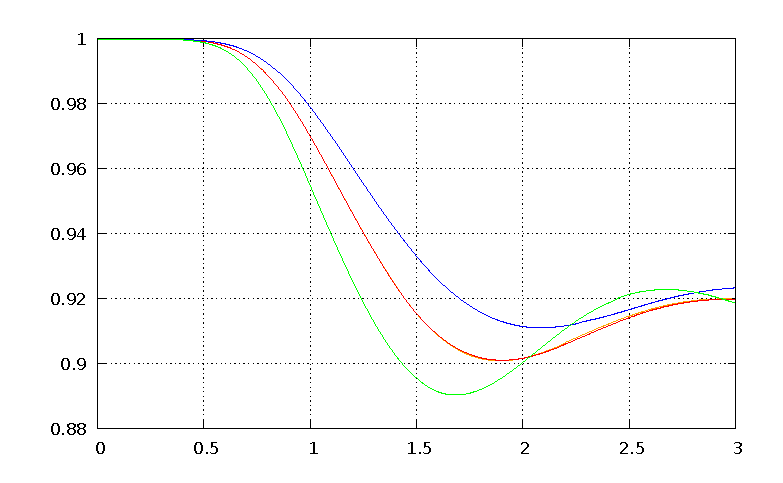
\includegraphics[width=.45\textwidth]
{figures/navier_stokes/2d_rising_bubble_sphericity.ps}
\caption[Navier--Stokes 2d rising bubble sphericity]
{A plot of the sphericity $\strikes$ over time for the simulation in
Figure~\ref{} for the explicit (orange), implicit (red), ALE (blue) and
antisymmetric (green) schemes.}
\label{fig:rising_bubble_2d_bulk_sphericity}
\end{figure}

\begin{figure}[htbp]
\centering
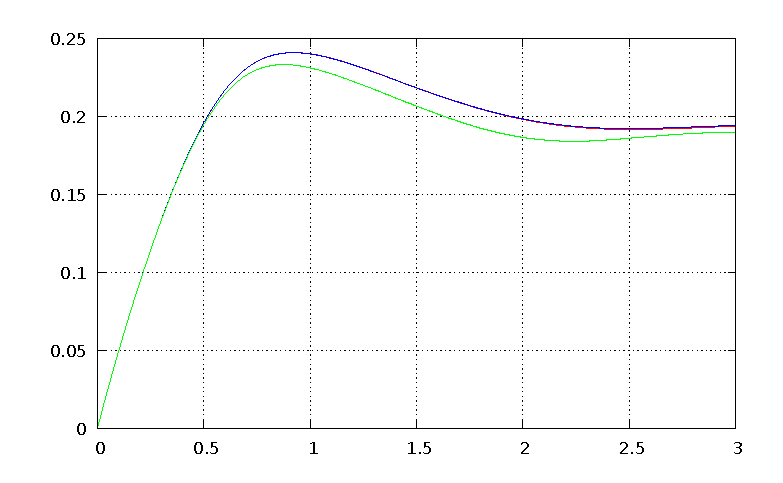
\includegraphics[width=.45\textwidth]
{figures/navier_stokes/2d_rising_bubble_rising_velocity.ps}
\caption[Navier--Stokes 2d rising bubble rising velocity]
{A plot of the rising velocity $V_c$ over time for the simulation in
Figure~\ref{} for the explicit (orange), implicit (red), ALE (blue) and
antisymmetric (green) schemes.}
\label{fig:rising_bubble_2d_bulk_rising_velocity}
\end{figure}

\begin{figure}[htbp]
\centering
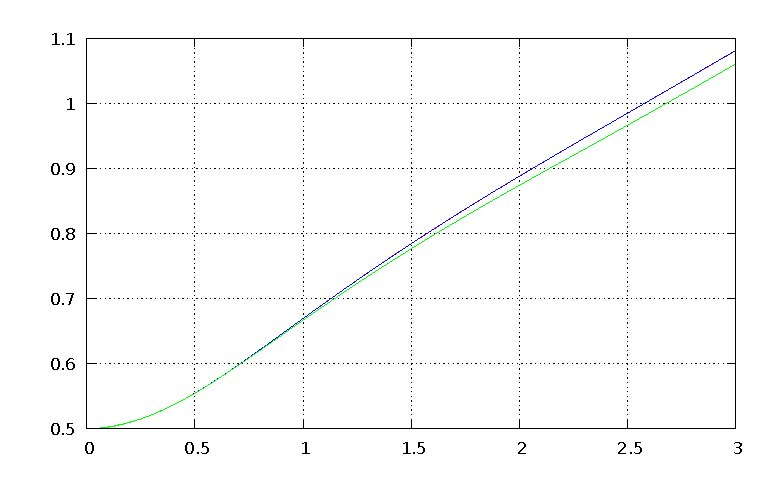
\includegraphics[width=.45\textwidth]
{figures/navier_stokes/2d_rising_bubble_barycenter.ps}
\caption[Navier--Stokes 2d rising bubble barycenter]
{A plot of the barycenter $z_c$ over time for the simulation in Figure~\ref{}
for the explicit (orange), implicit (red), ALE (blue) and antisymmetric (green)
schemes.}
\label{fig:rising_bubble_2d_bulk_barycenter}
\end{figure}

\begin{figure}[htbp]
\centering
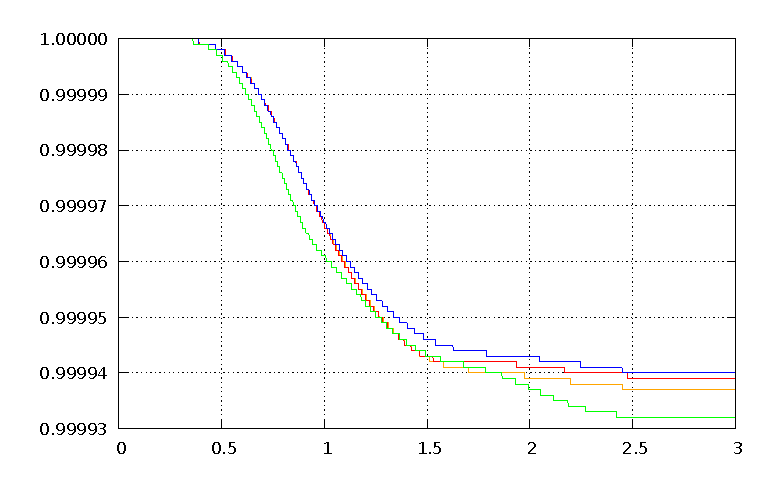
\includegraphics[width=.45\textwidth]
{figures/navier_stokes/2d_rising_bubble_inner_volume.ps}
\caption[Navier--Stokes 2d rising bubble inner area]
{A plot of the relative inner area
$\frac{\mathcal{L}^2(\Omega^m_-)}{\mathcal{L}^2(\Omega^0_-)}$
over time for the simulation in Figure~\ref{} for the explicit (orange),
implicit (red), ALE (blue) and antisymmetric (green) schemes.}
\label{fig:rising_bubble_2d_bulk_inner_volume}
\end{figure}